As mentioned in the earlier chapters, \velocty supports \matlab and Python's NumPy library. The \velocty backend takes VRIR as input and generates C++ code. We use PyVrir that is part of the Velociraptor toolkit generate VRIR from Python. However, no such tool exists to generate VRIR from \matlab to VRIR. The \mclab toolkit is a framework to aid static compilation of \matlab to different langauges. In order, to support the compilation of \matlab programs to C++ through \velocty, we implemented a VRIR generator using the \mclab toolkit. Section \ref{sec:comppipe} provided an overview of the compilation pipeline from \matlab to VRIR and then to C++. As mentioned in the section, the VRIR generator takes an input McSAF IR and generates the S-expression version of VRIR.

VRIR generation had challenges. The McSAF IR is a \matlab-specific IR whereas VRIR is designed to handle semantics of different langauges and thus contains flags to specify semantic information such as array layout, indexing scheme etc. We had to ensure the appropriate flags were set to correctly represent the semantics of \matlab. Moreover, VRIR is a strongly typed AST representation. Every expression node in VRIR has a type and shape information associated with it. McSAF does not explicitly hold this information and hence had to be determined during the compilation process. Additionally, \matlab functions do not need an explicit return statement for the output. When a return statement is explicitly provided, the parameters that need to be returned are not specified. This is because the output parameters are specified in the function signature. On the other hand, VRIR does not support output parameters and only supports output types. This difference in IR structure also had to be handled.

This chapter discusses the compilation of various nodes of the McSAF IR to VRIR, generation of the symbol table and how the types and shapes of expressions are determined.
\section{Mapping types}
In order to generate VRIR types, we require type and shape information as well as whether the symbol is real or complex. This information is obtained through the type analysis , the shape analysis and the isComplex analysis that were performed on Tamer. All variables and expressions are mapped to one of 5 VRIR types which are collectively known as VTypes.


\subsection{Scalar Type}
Scalar types are used for scalar symbols. In this case the shape of the symbol will have two dimensions each of size one. The scalar type also as a \textsf{ctype} flag which determines whether the symbol is real or complex. The symbol is considered to be real if the flag is set to zero and complex if it is set to one. The type of the data also needs to be specified in the generated VRIR. Types in \matlab are known as MClasses. Table \ref{tab:mclassList} gives a list of MClasses that are supported by the VRIR generator. Note that the VRIR generator does not support other MClasses such as \textsf{char}, unsigned integers and 16 and 8 bit integers. 
\begin{table}[htbp]
\centering
\begin{tabular}{|c|c|c|}
\hline
MClass  & VRIR Scalar Type & Description           \\ \hhline{|=|=|=|}
Logical & bool &Boolean type          \\ \hline
Int32   & int32 &32 bit Integer        \\ \hline
Int64   & int64 &64 bit Integer        \\ \hline
Float32 & float32 & 32 bit Floating point \\ \hline
Float64 & float64 & 64 bit Floating point \\ \hline
\end{tabular}
\caption[List of \matlab types]{The table lists the different \matlab types known as MClasses  that are supported by the VRIR generator and the Scalar types generated in VRIR.}
\label{tab:mclassList}
\end{table} 

Table \ref{tab:scalTypeMat} gives an example of VRIR for the scalar type from a \matlab variable \texttt{x}.  The example describes a scalar symbol that is of type \textsf{float64} and is \textsf{real}. 
\begin{table}[htbp]
\centering
\begin{tabular}{|l|l|}
\hline

\matlab &  Generated VRIR \\
\hline
{
\begin{lstlisting}[language=matlab,frame=none, numbers=none]
x = 0;
\end{lstlisting}
}
&
{
\begin{lstlisting}[language=lisp,frame=none, numbers=none]
(float64 :ctype 0)
\end{lstlisting}
} \\
\hline
\end{tabular}
\caption[Scalar Type example for \matlab]{The table shows an example of the generated scalar type for a scalar variable x in \matlab. }
\label{tab:scalTypeMat}
\end{table}
\subsection{Array Type}
The array type is used to represent types for \matlab arrays. Arrays can have two or more dimensions and at least one of the dimension sizes have to be greater than one. Note that although \matlab considers scalars to be 1x1 matrices, we make the distinction between scalars and arrays. Shape information is used to determine whether the symbol is an array or a scalar. Array types of VRIR contain information about the number of dimensions of the array and the array layout. The array layout can be \textsf{rowmajor}, \textsf{colmajor} and \textsf{strided}. However, in case of \matlab the layout is always \textsf{colmajor}. Array Types also contain a child node of scalar type. The scalar type holds information about the type of the array elements as well as whether they are \textsf{real} or \textsf{complex}. Table \ref{tab:arrTypeMat} gives an example of the generated array type. The example shows a variable array that is assigned to a 3x3 matrix of using the zeros builtin function. The generated VRIR array type contains a ndims attribute which is set to 2 since there are two dimensions, and the array layout attribute is set to colmajor since all arrays in \matlab are column major. Using the child scalar type node of the array type, we can determine that each element of the array is of type \textsf{float64} and that each element is \textsf{real}. 

\begin{table}[htbp]
\centering
\begin{tabular}{|l|l|}
\hline

\matlab &  Generated VRIR \\
\hline
{
\begin{lstlisting}[language=matlab,frame=none, numbers=none]
x = zeros(3,3);
\end{lstlisting}
}
&
{
\begin{lstlisting}[language=lisp,frame=none, numbers=none]
(arraytype :layout colmajor :ndims 2
		(float64 :ctype 0)
)
\end{lstlisting}
} \\
\hline
\end{tabular}
\caption[Array Type example for \matlab]{The table shows an example of the generated array type for an array variable x in \matlab. }
\label{tab:arrTypeMat}
\end{table}
\subsection{Void Type}
The void type is generally used as part of the Function type to convey the absence of the input or output parameters.
\subsection{Function Type}
\label{subsec:functypeMat}
Function types are associated with function definitions and function handles. They contain information about the types of the input and output parameters of the function. The \textsf{functype} node contains two child nodes, \textsf{intypes} and \textsf{outtypes}. Both nodes will have children that can be other VTypes such as scalar types, array types etc. The function types are part of the function node of VRIR. Table \ref{tab:funcTypeMat} gives an example of the Function type generated for the function babai. The function accepts two input parameters both of which are arrays and returns another array. The types of the input arguments are listed inside the intypes child whereas the output parameters are listed inside outtypes. Note that the body of the function is replaced by a statement inside chevrons which acts as a place holder. 
\begin{table}[htbp]
\centering
\begin{tabular}{|l|l|}
\hline

\matlab &  Generated VRIR \\
\hline
{
\begin{lstlisting}[language=matlab,frame=none, numbers=none]
function [z_hat] = babai(R,y) 
<Function Body> 
end;
\end{lstlisting}
}
&
{
\begin{lstlisting}[language=lisp,frame=none, numbers=none]
(functype
	(intypes
		( arraytype :layout colmajor :ndims 2
			(float64 :ctype 0)
		)
		( arraytype :layout colmajor :ndims 2
			(float64 :ctype 0)
		)
	)
	(outtypes
		( arraytype :layout colmajor :ndims 2
			(float64 :ctype 0)
		)
	)
)
\end{lstlisting}
} \\
\hline
\end{tabular}
\caption[Func Type example for \matlab]{The table shows an example of the generated func type for the function babai in \matlab. }
\label{tab:funcTypeMat}
\end{table}
\subsection{Tuple Type}
Tuple types are used to define data structures which can have data of different types. Table \ref{tab:tupletype} gives an example of the tuple type. The table shows a function call to \textsf{spqr} which has multiple returns. The function call expression as well as the expression on the LHS will both have tuple types. In this case the tuple type specifies that the two variables being returned have VTypes, scalar type and array type respectively. 
\begin{table}[htbp]
\centering
\begin{tabular}{|l|l|}
\hline
\matlab &  generated VRIR\\
\hline
{
\begin{lstlisting}[language=matlab,frame=none, numbers=none]
[nc, r]  = spqr(a,tol,maxrc)
\end{lstlisting}
}
&
{
\begin{lstlisting}[language=lisp,frame=none, numbers=none]
(tupletype
	(float64 :ctype 0)
	(arraytype :layout colmajor :ndims 2
		(float64 :ctype 0)
	)
)
\end{lstlisting}
} \\
\hline
\end{tabular}
\caption[Example of the Tuple Type]{The table gives an example of a call to a function with multiple returns in \matlab and the equivalent VRIR tuple type that is generated.}
\label{tab:tupletype}
\end{table}

\subsection{Domain Type}
The domain type is associated with the domain expression explained in Subsection \ref{subsec:domainExprfront}. Domain expressions themselves are only associated with For or parallel For loop statements. Domain types specify the types of all the iterator variables of the loop statements. The domain type has an attribute ndims which specifies the number of iteration variables of the loop. In case of \matlab, there can only be one iteration variable per loop. Listing \ref{lst:domaintype} gives an example of a domain type for a single iteration variable that is of type \textsf{float64}. 
\begin{lstlisting}[language=lisp, label={lst:domaintype}, caption={An example of the domain type in VRIR. }]
(domaintype :ndims 1 (float64 :ctype 0))
\end{lstlisting}

\section{Symbol Table}
The symbol table contains a list of symbols that are defined inside a function in VRIR. The table contains the name and the type of each symbol. Moreover, there is a unique id associated with every symbol using which it is referenced in the function. There is a symbol table for every function in VRIR. Listing \ref{lst:symtab} gives an example of a symbol table. The symbol table contains a set of sym nodes each having a unique id. For example, the sym node with id 5 on line 2 is the symbol par which is of type \textsf{float64}. The VRIR generator adds symbols when it comes across new symbols while traversing the function's abstract syntax tree. The VRIR code for the symbol table is then generated after the function body.
\begin{lstlisting}[language=lisp, label={lst:symtab}, caption={Symbol table in VRIR}]
(symtable
	(sym :id 5 :name par 
		(float64 :ctype 0)) 
	(sym :id 0 :name R 
		( arraytype :layout colmajor :ndims 2
			(float64 :ctype 0)
		)
	) 
	(sym :id 4 :name k 
		(float64 :ctype 0)
	) 
	(sym :id 3 :name n 
		(float64 :ctype 0)
	) 
)
\end{lstlisting}

\section{Generating the Module VRIR node}
The root node of VRIR is the module. Every valid VRIR must contain the module as its root node. The module contains an attribute, \textsf{indexing}, which defines the type of array indexing used. The attribute can have two values \textsf{0} indicating zero indexing and \textsf{1} indicating one indexing. Since the \matlab arrays are one indexed, the indexing attribute is always set to \textsf{1}. The module node also contains a name attribute specifying the name of the module. Additionally, it contains a \textsf{fns} child node which itself has multiple function nodes as its children. Listing \ref{lst:moduleGen} gives an example of the module node of VRIR. The name of the module is babai and the indexing attribute is set to one. 
\begin{lstlisting}[language=lisp, label={lst:moduleGen}, caption={The listing gives an example of a VRIR module that is generated by the VRIR generator.}]
(module :name babai :indexing 1
	(fns
		<functions> 
	)
)

\end{lstlisting}

\section{Handling functions}
\label{sec:funcGen}
\matlab programs can have one or more functions. As mentioned in Section \ref{sec:execModel}, the user specifies the entry point function using which a callgraph containing functions that are reachable from the entry point function is generated. All of the functions that are part of the callgraph are compiled to VRIR. The function node in VRIR has multiple children all of which are required to generate the C++ code for the function. 
\begin{itemize}
\item Name : The function name represents the name of the function.
\item Arglist : The arglist is a list of integers which are the Ids of the input arguments in the symbol table.
\item Func type : The Func type gives information about about the types and shapes of the input and output parameters of the function. 
\item Body : The body represents the body of the function. It consists of a list of statements. 
\item Symbol Table : Contains information about the symbols used in the function. 
\end{itemize}
The Table \ref{tab:functionGen} gives an example of the function VRIR node for the \matlab function \textsf{babai}. The function has two input arguments and one output parameter. Thus the intypes has two Vtype nodes and the outtype has a single VType node. Moreover, Since there are two input arguments, the arglist has two arg nodes. 
\begin{table}[htbp]
\centering
\begin{tabular}{|l|l|}
\hline

\matlab &  Generated VRIR \\
\hline
{
\begin{lstlisting}[language=matlab,frame=none, numbers=none]
function [z_hat] = babai(R,y) 
<Function Body> 
end;
\end{lstlisting}
}
&
{
\begin{lstlisting}[language=lisp,frame=none, numbers=none]
(function babai
	(functype
		(intypes
			( arraytype :layout colmajor :ndims 2
				(float64 :ctype 0)
			)
			( arraytype :layout colmajor :ndims 2
				(float64 :ctype 0)
			)
		)
		(outtypes
			( arraytype :layout colmajor :ndims 2
				(float64 :ctype 0)
			)
		)
	)
	(arglist
		(arg :id 0)
		(arg :id 1)
	)
	(body
		<body>
	)
	(symtable
		<Symbol Table>
	)
)
\end{lstlisting}
} \\
\hline
\end{tabular}
\caption[Function example for \matlab]{The table shows an example of the generated Function VRIR node  for the function babai in \matlab. }
\label{tab:functionGen}
\end{table}

\section{Mapping statements}
Many of the statements in \matlab have equivalent VRIR statement nodes. However, some require additional processing while generating their VRIR equivalent. 

\subsection{Assignment Statements}
Assignment statements in \matlab are compiled to the assignment statement node in VRIR. The assignment statement node of VRIR contains two child nodes, \textsf{lhs} and \textsf{rhs}. As the names suggest, the left hand side expression of assignment statement in \matlab is compiled to an expression inside the \textsf{lhs} node and the right hand side expression is compiled to an expression inside the \textsf{rhs} node. Table \ref{tab:assignGen} gives an example of a \matlab statement that is compiled to a assignment statement node in VRIR. The left hand side is a scalar variable \textsf{n} and the right hand side is a call to the function \textsf{length}. 
\begin{table}[htbp]
\centering
\begin{tabular}{|l|l|}
\hline

\matlab &  Generated VRIR \\
\hline
{
\begin{lstlisting}[language=matlab,frame=none, numbers=none]
n = length(y)
\end{lstlisting}
}
&
{
\begin{lstlisting}[frame=none, numbers=none]
(assignstmt
	(lhs
		(name :id 3
			(float64 :ctype 0)
		)
	)
	(rhs
		(fncall :fnname length
			(float64 :ctype 0)
			(args
				(name :id 1
					( arraytype :layout colmajor :ndims 2
						(float64 :ctype 0)
					)
				)
			)
		)
	)
)
\end{lstlisting}
} \\
\hline
\end{tabular}
\caption[Assignment Statement example in \matlab and VRIR]{The table shows an example of the generated assignment statement VRIR node a statement in \matlab.}
\label{tab:assignGen}
\end{table}

\subsubsection{Copy statements}
We define copy statements as assignment statement where both the left hand side and right hand side are array variables. Listing \ref{lst:copyStmtGen} gives an example of a copy statement in \matlab. An array \textsf{B} is copied into another array \textsf{A}. According to \matlab semantics, a deep copy\footnote{The data is actually copied from one array to the other} has to be performed. However, VRIR supports a reference copy\footnote{Only the reference of the array is copied to the other array. Thus both arrays are referring to the same data.}. Hence an explicit copy function call has to be added. We make use the copy library function of VRIR that is explained in Subsection \ref{subsec:paramGen}.  The right hand side is added as an argument of the copy function and the function call itself becomes the rhs of the assignment statement\footnote{As a future work we would like to implement an analysis to remove copies where they are not required.}.
\begin{lstlisting}[float,language=lisp, label={lst:copyStmtGen}, caption={The listing gives an example of a copy statement in \matlab. }]
B = zeros(3,3);
A = B;
\end{lstlisting}
 Table \ref{tab:copyGen} gives an example of the copy statement. The array \textsf{A} is copied to another array \textsf{x}. In the generated code a library call expression representing the call to the copy function on the rhs. 
\begin{table}[htbp]
\centering
\begin{tabular}{|l|l|}
\hline

\matlab &  Generated VRIR \\
\hline
{
\begin{lstlisting}[language=matlab,frame=none, numbers=none]
 x=A;
\end{lstlisting}
}
&
{
\begin{lstlisting}[frame=none, numbers=none]
(assignstmt
	(lhs
		(name :id 1
			( arraytype :layout colmajor :ndims 2
				(float64 :ctype 0)
			)
		)
	)
	(rhs
		(libcall :libfunc copy
			(args
				(name :id 0
					( arraytype :layout colmajor :ndims 2
						(float64 :ctype 0)
					)
				)
			)
		
		)
	)
)
\end{lstlisting}
} \\
\hline
\end{tabular}
\caption[Copy Assignment Statement example in \matlab and VRIR]{The table shows an example of the generated copy assignment statement VRIR node a statement in \matlab.}
\label{tab:copyGen}
\end{table}

\subsection{For and Parallel For Statements}
The \matlab For statement is mapped to the For statement node of VRIR and the Parfor statement to the parallel For in VRIR. The McSAF IR does not have a separate Parfor node. Instead the For statement node contains a boolean flag which when set to true implies that the node is a Parfor statement. The flag when set to false implies that the node is a for statement. 

The For statement node in VRIR has 3 children. The \textsf{body} node represents the list of statements that make up the loop body. \textsf{Itervars} is an array of the symbol table ids of the iteration variables of the loops. In case of \matlab, there are only be one iteration variable. The \textsf{loopdomain} contains a domain expression which in turn defines the bounds of the loop. Table \ref{tab:forGen} gives an example of the for statement in \matlab and the equivalent VRIR \textsf{for} statement node. The iteration variable is \textsf{k} and the loops bounds are \textsf{n-1} to \textsf{1}. The step value is \textsf{-1}.
\begin{table}[htbp]
\centering
\begin{tabular}{|l|l|}
\hline

\matlab &  Generated VRIR \\
\hline
{
\begin{lstlisting}[language=matlab,frame=none, numbers=none]
for k=n-1:-1:1
	<Loop Body>
end;
\end{lstlisting}
}
&
{
\begin{lstlisting}[frame=none, numbers=none]
(forstmt
	(itervars
		(sym :id 4
  		)
	)
	(loopdomain
  		(domain
   			( domaintype :ndims 1 (float64 :ctype 0))
			(range :exclude %0
   				(start
   					(minus
   						(float64 :ctype 0)
							(lhs
   								(name :id 3
   									(float64 :ctype 0)
								)
							)
							(rhs
   								(realconst :dval 1
									(float64 :ctype 0)
								)
							)
					)
				)
				(step
					(negate
   						(float64 :ctype 0)
						(realconst :dval 1
							(float64 :ctype 0)
						)
					)
				)
				(stop
					(realconst :dval 1
						(float64 :ctype 0)
					)
				)
			)
		)
	)
	(body 
		<Loop Body>
	)
)
\end{lstlisting}
} \\
\hline
\end{tabular}
\caption[For Statement example in \matlab and VRIR]{The table shows an example of the generated For statement VRIR node a statement in \matlab.}
\label{tab:forGen}
\end{table}

The parallel for statement node in VRIR also contains the three child nodes mentioned above. However, it also contains an additional node, \textsf{shared}. The \textsf{shared} node contains a list of symbol table ids of the variables that are shared across loop iterations. 

\subsection{Return Statement}
The return statement in \matlab is mapped to the return statement node in VRIR. However, the return statement in \matlab and therefore the return statement node in McSAF IR, does not specify the variables to be returned. This is because the function node of McSAF IR contains the information about the output parameters. But the function node in VRIR does not have a child node for the output parameters. Hence to allow the VRIR backend to determine the variables that need to be returned, we explicitly add the output parameters specified by the McSAF IR function node to the return statement node of VRIR. Table \ref{tab:returnGen} gives an example of the return statement. The \matlab function has a single output parameter \textsf{z\_hat}. However, the return does not specify the fact that \textsf{z\_hat} is a return parameter. Hence it has to explicitly added, as we can observe in the VRIR code in the second column. 
\begin{table}[htbp]
\centering
\begin{tabular}{|l|l|}
\hline

\matlab &  Generated VRIR \\
\hline
{
\begin{lstlisting}[language=matlab,frame=none, numbers=none]
function z_hat = babai(R,y) 
	<Function Body> 
	return;
end
\end{lstlisting}
}
&
{
\begin{lstlisting}[frame=none, numbers=none]
(returnstmt
	(exprs
		(name :id 2
			(arraytype :layout colmajor :ndims 2
				(float64 :ctype 0)
			)
		)
	)
)
\end{lstlisting}
} \\
\hline
\end{tabular}
\caption[Return Statement example in \matlab and VRIR]{The table shows an example of the generated Return statement VRIR node a statement in \matlab.}
\label{tab:returnGen}
\end{table}

In \matlab, a function need not have an explicit return statement. All the output parameters are returned to the caller once the end of the function is reached. However, for reasons mentioned above, we need a return statement in VRIR. Hence a return statement is explictly added along with the output parameters. 

In some cases the return statement may not be accessible through all paths. For example, if a return statement is present inside a \textsf{if} block, the return statement will be executed only if the \textsf{if} condition is true. In such cases, we add the output parameters to the existing return statement and also add a return statement at the end of the function body. 

Table \ref{tab:retList} gives a list of possible cases for the return statement in a \matlab function and the actions that are taken for each case. 
\begin{table}[htbp]
\centering
\begin{tabular}{|c|c|}
\hline
Status of Return statement in \matlab                                                               & Action taken                                                                                                                                                                                      \\ \hhline{|=|=|}
No Return statement present.                                                                       & \begin{tabular}[c]{@{}c@{}}Statement explicitly added at \\ the end of the function body\\ along with return variables.\end{tabular}                                                              \\ \hline
\begin{tabular}[c]{@{}c@{}}Return statement present. Not accessible \\ from all paths\end{tabular} & \begin{tabular}[c]{@{}c@{}}Statement explicitly added at \\ the end of the function body \\ along with return variables\\ Return variables added to \\ existing return statement.\end{tabular} \\ \hline
\begin{tabular}[c]{@{}c@{}}Return statement present. Accessible from\\ all paths\end{tabular}      & \begin{tabular}[c]{@{}c@{}}Return variables added to\\ existing return statement.\end{tabular}                                                                                                    \\ \hline
\end{tabular}
\caption[List of cases for return statements in \matlab]{The table gives a list of possible cases for the presence of the return statement in a \matlab function and the subsequent actions taken for each case. }
\label{tab:retList}
\end{table}
\subsection{If Statement}
The If statement in \matlab is compiled to the If statement node in VRIR. The If statement in VRIR has three child nodes. The test expression contains the If condition, the If child contains the list of statements inside the If block and the else child contains the list of statement inside the else block. Table \ref{tab:ifGen} gives an example of the If statement. 
\begin{table}[htbp]
\centering
\begin{tabular}{|l|l|}
\hline

\matlab &  Generated VRIR \\
\hline
{
\begin{lstlisting}[language=matlab,frame=none, numbers=none]
	if <test condition>
		<If Block>
	else 
		<Else Block>
	end;
\end{lstlisting}
}
&
{
\begin{lstlisting}[frame=none, numbers=none]
(ifstmt
	(test
		<test condition>
	)
	(if 
		<If block>
	)
	( else 
		<Else block>
	)
)

\end{lstlisting}
} \\
\hline
\end{tabular}
\caption[If Statement example in \matlab and VRIR]{The table shows an example of the generated If statement VRIR node a statement in \matlab.}
\label{tab:ifGen}
\end{table}
\subsection{While Statement}
Similar to the If statement, the While statement in \matlab is mapped to the While statement node in VRIR. The While statement node in VRIR contains two child nodes. A test node while holds the While condition and the body node which holds the statements of the loop body. 
\begin{table}[htbp]
\centering
\begin{tabular}{|l|l|}
\hline

\matlab &  Generated VRIR \\
\hline
{
\begin{lstlisting}[language=matlab,frame=none, numbers=none]
	while <test condition>
		<While Body>
	end;
\end{lstlisting}
}
&
{
\begin{lstlisting}[frame=none, numbers=none]
(whilestmt
	(test
		<test condition>
	)
	(body 
		<While Body>
	)
)

\end{lstlisting}
} \\
\hline
\end{tabular}
\caption[While Statement example in \matlab and VRIR]{The table shows an example of the generated While statement VRIR node a statement in \matlab.}
\label{tab:whileGen}
\end{table}

\subsection{Break and Continue statements}
The break and continue statements in \matlab are compiled to the break continue statement nodes in VRIR respectively. 

\section{Mapping Expressions}
Similar to statements, many expressions in \matlab have equivalent expression nodes in VRIR. However, every expression node must have a VType associated with it. This is not the case with the McSAF IR. Hence the VType of each expression is required to be calculated during code generation. 

\subsection{Name Expressions}
Name expressions in \matlab can either mean a variable or a call to a function with arguments. In the case of variables, a name expression is generated in VRIR. A function call expression is generated if the expression represents a call to a function. If expression is the first occurrence of the variable, an entry in symbol table is also made. The name expression contains an id attribute. The id attribute value represents the id of the variable in the symbol table. Table \ref{tab:nameGen} gives an example of a variable in \matlab and its equivalent name expression node in VRIR. The example shows the generated name expression for variable A. The id of the variable in the symbol table is 10. The symbol table entry for the variable is also shown.
\begin{table}[htbp]
\centering
\begin{tabular}{|l|l|}
\hline

\matlab &  Generated VRIR \\
\hline
{
\begin{lstlisting}[language=matlab,frame=none, numbers=none]
A
\end{lstlisting}
}
&
{
\begin{lstlisting}[language=lisp,frame=none, numbers=none]
;; Generated Name expression

(name :id 10)

;; Entry in symbol table.
(sym :id 10 :name A 
	(float64 :ctype 0)
)
\end{lstlisting}
} \\
\hline
\end{tabular}
\caption[Name Expression example for \matlab]{The table shows an example of the generated name expression node for a variable A in \matlab. The entry of the variable in the symbol table is also shown. }
\label{tab:nameGen}
\end{table}
\subsection{Paramaterized Expressions}
\label{subsec:paramGen}
Parameterized experssions can be mapped to many different nodes in VRIR depending on their semantics. In \matlab, a parameterized expression can be an array index operation or a function call. The kind analysis\cite{Doherty:2011:KAM:2076021.2048077} is  used to differentiate between function calls and array index operations. 
\subsubsection{Index Expressions}
If the parameterized expression in McSAF represents an index operation, the VRIR generator compiles the expression to an index expression. Table \ref{tab:indexGen} gives an example of an array index operation in \matlab and the equivalent VRIR code that was generated. The index operation has two indices. The first one is a simple numeric index \textsf{k},  whereas the second one is a slice index and hence specifies a range of index values starting from \textsf{k+1} to \textsf{n}. The VRIR index expression node  has an \textsf{arrayid} attribute which holds the id of the array inside the symbol table. In the example, the array id 0 refers to the array R. The copyslice flag whether the values of set of indices reprented by the indices have to be copied to a new array. The \textsf{indices} child node of array holds the set of indices of the index operation. Each child node is of type index. Note that this node is different from the index expression node. The index node has two attributes. The \textsf{boundschecks} attribute indicates whether array bounds checks need to be added for the index. The \textsf{negative} attribute indicates whether the index value can be negative. In case of \matlab, the \textsf{boundscheck} attribute  is set to \textsf{\%1} to include bounds checks and the \textsf{negative} attribute is set to \textsf{\%0} to indicate that negative indexing is not supported. 
\begin{table}[htbp]
\centering
\begin{tabular}{|l|l|}
\hline

\matlab &  Generated VRIR \\
\hline
{
\begin{lstlisting}[language=c,frame=none, numbers=none]
R(k,(k+1):n)
\end{lstlisting}
} 
&
{
\begin{lstlisting}[language=lisp,frame=none, numbers=none]
(index :arrayid 0 :copyslice %1
	( arraytype :layout colmajor :ndims 2
		(float64 :ctype 0))
	(indices
		(index :boundscheck %1 :negative %0
			(name :id 4
				(float64 :ctype 0)
			)
		)
		(index :boundscheck %1 :negative %0
			(range :exclude %0
				(start
					(plus
						(float64 :ctype 0)
						(lhs
							(name :id 4
								(float64 :ctype 0)
							)
						)
						(rhs
							(realconst :dval 1
								(float64 :ctype 0)
							)
						)
					)
				)
				(stop
					(name :id 3
						(float64 :ctype 0)
					)
				)
			)
		)
	)
)
\end{lstlisting}
}
\\
\hline
\end{tabular}
\caption[Index Expression Generation Example]{The table shows a \matlab index operation with a slice operation that is compiled VRIR}
\label{tab:indexGen}
\end{table}
\subsubsection{Function Call Expressions}
Parameterized expressions that are calls to functions in \matlab can be divided into four broad categories: operators, library calls, allocation function calls and miscellaneous function calls. 

Operators include binary and unary operators such as plus, minus, unary minus etc. Although the McSAF IR does have nodes for all the operators, Tamer converts the operators to function calls when generating TameIR and Tamer+ keeps them as function calls. In case of operations on scalars, we convert the parameterized expressions representing operators to equivalent operators in VRIR. For some of these operators, if at least one of the operands are arrays, a libcall expression is generated. Table \ref{tab:opGen} gives a list of \matlab operators  and the VRIR nodes that are generated. If the last column, array operands, has a `yes', the VRIR node is also generated for the array operands. 
\begin{table}[htbp]
\centering
\begin{tabular}{|c|c|c|}
\hline
Matlab function & VRIR Node & Array Operands \\ \hhline{|=|=|=|}
plus            & plus   & No   \\ \hline
minus           & minus  & No   \\ \hline
rdivide         & div    & No   \\ \hline
mtimes          & mmult  & No   \\ \hline
times           & mult   & No   \\ \hline
or              & or     & Yes   \\ \hline
eq              & eq     & Yes   \\ \hline
le              & leq    & Yes   \\ \hline
ge              & geq    & Yes   \\ \hline
lt              & lt     & Yes   \\ \hline
gt              & gt     & Yes   \\ \hline
uminus          & negate & Yes   \\ \hline
not             & negate & Yes   \\ \hline
\end{tabular}
\caption[List of operators in \matlab and their equivalent VRIR nodes]{ The table list the operators in \matlab and the equivalent VRIR nodes that are generated. }
\label{tab:opGen}
\end{table}

Table \ref{tab:opEx} gives an example of a plus operator in \matlab which has two operand expressions that are converted to the plus expression in VRIR. All other operators have a similar structure in VRIR. 
\begin{table}[htbp]
\centering
\begin{tabular}{|l|l|}
\hline
\matlab &  Generated VRIR\\
\hline
{
\begin{lstlisting}[language=matlab,frame=none, numbers=none]
<op1> + <op2>;
\end{lstlisting}
}
&
{
\begin{lstlisting}[language=lisp,frame=none, numbers=none]
(plus
	(float64 :ctype 0)
	(lhs
		<op2>
	)
	(rhs
		<op2>
	)
)
\end{lstlisting}
} \\
\hline
\end{tabular}
\caption[Example of operators in \matlab and VRIR]{The table shows an example of a plus operator in \matlab that is converted to a plus expression node in VRIR}
\label{tab:opEx}
\end{table}

As mentioned, operations on arrays are compiled to library call operations in VRIR. Additionally, operators that can only take array operands such as matrix multiplication, transpose, matrix division among others, are also supported through library call expressions. Library call expressions also support some other functions that are commonly used in numerical and scientific computing and hence many of those functions are also compiled to library call expressions. Table \ref{tab:libCallGen} lists the scientific functions that are supported by the \textsf{libcall} expression. 
\begin{table}[htbp]
\centering
\begin{tabular}{|c|c|}
\hline
Library Functions & Description           \\ \hline
Sqrt              & Square root           \\ \hline
Log2              & Log with base 2       \\ \hline
Log10             & Log with base 10      \\ \hline
Expe              & exponent of e         \\ \hline
Exp10             & exponent of 10        \\ \hline
Sin               & Trigonometric Sin     \\ \hline
Cos               & Trigonometric Cosine  \\ \hline
Tan               & Trigonometric tangent \\ \hline
Asin              & Inverse sin           \\ \hline
Acos              & Inverse cosine        \\ \hline
Atan              & Inverse tangent       \\ \hline
Pow               & power function        \\ \hline
Sum               & Sum function          \\ \hline
Prod              & Product function      \\ \hline
Atan2             & Arc Tangent           \\ \hline
Abs               & Absolute value        \\ \hline
Min               & Min function          \\ \hline
Max               & Max Function          \\ \hline
Mean              & Mean function         \\ \hline
Copy              & Copy function         \\ \hline
Mmult              & Matrix Multiplication         \\ \hline
Mrdiv              & Matrix right division         \\ \hline
Mldiv              & Matrix left division         \\ \hline
Div              & Element wise array division         \\ \hline
Mult              & Element wise array multiplication         \\ \hline
Plus              & Element wise array addition         \\ \hline
Minus              & Element wise array subtraction         \\ \hline
\end{tabular}
\caption[List of functions supported by library call expressions]{The table lists the functions supported by the library call expression in VRIR.}
\label{tab:libCallGen}
\end{table}

Calls to functions like \textsf{zeros} and \textsf{ones} which are used to create arrays in \matlab are compiled to the alloc expressions in VRIR. Table \ref{tab:allocGen} gives an example of a \matlab function \textsf{zeros} and the VRIR alloc expression that was generated. The alloc expression contains a \textsf{func} attribute which defines the name of the function. It takes three values, \textsf{zeros}, \textsf{ones} and \textsf{empty}. The \textsf{zeros} function creates an array and initialises all elements to zero, ones creates an array and initialises all elements to one and \textsf{empty} creates an uninitialised array. \matlab does not support the \textsf{empty} function and hence the VRIR generator only generates the \textsf{ones} and the \textsf{zeros} function. The alloc expression also has a child node \textsf{args} which holds the input arguments of the function. 
\begin{table}[htbp]
\centering
\begin{tabular}{|l|l|}
\hline
\matlab &  Generated VRIR\\
\hline
{
\begin{lstlisting}[language=matlab,frame=none, numbers=none]
zeros(m,n);
\end{lstlisting}
}
&
{
\begin{lstlisting}[language=lisp,frame=none, numbers=none]
(alloc :func zeros
	( arraytype :layout colmajor :ndims 2
		(float64 :ctype 0)
	)
	(args
		(name :id 2
   			(float64 :ctype 0)
		)
		(name :id 4
   			(float64 :ctype 0)
		)
	)
)
\end{lstlisting}
} \\
\hline
\end{tabular}
\caption[Example of a zeros function call in \matlab and equivalent VRIR code]{The table gives an example of the zeros function call in \matlab and the equivalent alloc expression that is generated in VRIR.}
\label{tab:allocGen}
\end{table}

Function calls which do not qualify as library call expressions or alloc expressions are compiled to the function call expression node in VRIR. These include calls to user-defined functions as well as builtin functions that are not supported by alloc or library call expressions. 

In \matlab arguments to functions are passed by value. On the other hand, in VRIR, arguments are passed by reference. Hence in order to generate code that matches \matlab semantics, we add calls to the library call function \textsf{copy} for every array argument that is passed to a call to a user-defined function. Builtin implementations ensure that a input arguments are copied if they have to be written to and hence no function calls to \textsf{copy} are generated. Table \ref{tab:funcGen} gives an example of a user-defined function gauss that is compiled to a function call expression in VRIR. The name of the function is defined by the attribute \textsf{fnname}. The args child node contains the input arguments to the function. The arguments are copied by adding a call to the library call function \textsf{copy}.
\begin{table}[htbp]
\centering
\begin{tabular}{|l|l|}
\hline
\matlab &  Generated VRIR\\
\hline
{
\begin{lstlisting}[language=matlab,frame=none, numbers=none]
gauss(n,m)
\end{lstlisting}
}
&
{
\begin{lstlisting}[language=lisp,frame=none, numbers=none]
(fncall :fnname gauss
	(float64 :ctype 0)
	(args
		(libcall :libfunc copy 
			(float64 :ctype 0) 
			(args 
				(name :id 4
   					(float64 :ctype 0)
				)
			)
		)
		( libcall :libfunc copy 
			(float64 :ctype 0) 
			(args 
				(name :id 11
   					(float64 :ctype 0)
				)
			)
		)
	)
)
\end{lstlisting}
} \\
\hline
\end{tabular}
\caption[Example of a function call in \matlab compiled to a function call expression]{The table gives an example of a user-defined function call in \matlab and the equivalent function call expression that is generated in VRIR.}
\label{tab:funcGen}
\end{table}
\subsection{Matrix Expressions}
Matrix expressions in \matlab are used to represent multiple expressions and are often are found on the left hand side of an assignment statement where the right hand side is a call to a function with multiple output parameters. Matrix expressions are compiled to tuple expressions in VRIR. Table \ref{tab:matrixGen} gives an example of a matrix expression and the equivalent tuple expression. A tuple type is generated for a tuple expression which holds the types for each of the expressions inside the tuple expression. The tuple expression also holds a \textsf{elem} child node which holds the expressions of the matrix expression. In this case, the matrix expression contains two name expressions. Note the generated VRIR code only depicts the left hand side of the assignment statement.
\begin{table}[htbp]
\centering
\begin{tabular}{|l|l|}
\hline
\matlab &  generated VRIR\\
\hline
{
\begin{lstlisting}[language=matlab,frame=none, numbers=none]
[nc, r]  = spqr(a,tol,maxrc)
\end{lstlisting}
}
&
{
\begin{lstlisting}[language=lisp,frame=none, numbers=none]
(tuple
	(tupletype
		(float64 :ctype 0)
		(arraytype :layout colmajor :ndims 2
			(float64 :ctype 0)
		)
	)
	(elems
		(name :id 3
			(float64 :ctype 0)
		)
		(name :id 8
   			( arraytype :layout colmajor :ndims 2
				(float64 :ctype 0)
			)
		)
	)
)
\end{lstlisting}
} \\
\hline
\end{tabular}
\caption[Example of a matrix expression in \matlab with the equivalent VRIR code]{The table gives an example of a matrix expression in \matlab and the equivalent VRIR tuple expression that is generated.}
\label{tab:matrixGen}
\end{table}
\subsection{Literal Expressions}
Literal expressions are expressions in \matlab holding constant value. There are three types of literal expression in \matlab: FP literal expressions which represent the floating point constants, Int literal expressions which represent integer constants and string literal expressions which represent strings. Since VRIR does not support strings, the VRIR generator does not support the string literal expression. Both the Fp literal expression and the Int literal expressions are compiled to the constant expression in VRIR.

 Table \ref{tab:constGen} gives an example of the constant expression in VRIR that is generated from a constant value in \matlab. The constant expression in VRIR has a \textsf{dval} attribue which specifies a floating point constant value. Whether the value is 64 bit or 32 bit can be determined by checking the type of the expression. In case of Int literal expressions, the \textsf{ival} attribute is used. 
\begin{table}[htbp]
\centering
\begin{tabular}{|l|l|}
\hline
\matlab &  generated VRIR\\
\hline
{
\begin{lstlisting}[language=matlab,frame=none, numbers=none]
 oldcap = 0;
\end{lstlisting}
}
&
{
\begin{lstlisting}[language=lisp,frame=none, numbers=none]
(realconst :dval 0
	(float64 :ctype 0)
)
\end{lstlisting}
} \\
\hline
\end{tabular}
\caption[Example of a FP literal in \matlab with the equivalent VRIR code]{the table gives an example of a FP literal expression in \matlab and the equivalent VRIR constant expression that is generated.}
\label{tab:constGen}
\end{table}
\subsection{Range Expressions} 
\label{subsec:range}
Range expressions are used to define a range of values. They hold three expressions, start, stop and step. The start expression refers to the start of the range, the stop to the end of the range and the step refers to the interval between two consecutive values. A range expression is compiled to a range node in VRIR. A range node also has three expressions, start, stop and step. The range node represents a range from the start expressions value to the stop expression value with intervals of the step expression value. Whether the stop expression value is included in the range is determined using the exclude attribute. If the exclude attribute is set to \textsf{\%1} the stop expression value is excluded and the stop expression value is included when the exclude attribute is set to \textsf{\%0}. In case of \matlab, since the stop expression value is always included, the exclude attribute is always set to \textsf{\%0}. The step expression value is optional and defaults to 1 if not specified. Ranges are used for two reasons, one to represent loop bounds and other to represent an array slice in an index operation. Listing \ref{lst:rangeGen} gives an example of a range node in VRIR. The exclude flag is set to \textsf{\%0} and hence the stop expression value will be included. 
\begin{lstlisting}[float,language=matlab, label={lst:rangeGen}, caption={Example of a Range in VRIR}]
(range :exclude %0
	(start
		<Start Expression>
	)
	(step
		<Step Expression>		
    )
	(stop
		<Stop Expression>
	)
)
\end{lstlisting}

\subsection{Domain Expressions}
\label{subsec:domainExprfront}
Domain expressions are used in \textsf{for} statements to specify the loop bounds. Domain expressions can support multiple loop bounds, one for each iteration variable. However \matlab only allows a single iteration variable for a loop and hence only one set of loop bounds exist inside a domain expression for \matlab. The VType of the domain expression is the domain type which holds the VTypes of all the iteration variables of the loop. The loop bounds are represented by ranges described in Subsection \ref{subsec:range}. 

Table \ref{tab:domainGen} gives an example of the domain expression that is generated as part of the for statement in VRIR. The Domain expression has a domain type and a single range for the iteration variable. The range starts from 1 and stops at \textsf{na}. Since the exclude attribute is not set, the stop value is included in the range.
\begin{table}[htbp]
\centering
\begin{tabular}{|l|l|}
\hline
\matlab &  Generated VRIR\\
\hline
{
\begin{lstlisting}[language=matlab,frame=none, numbers=none]
 for ii = 1:na
	<Loop Body>
 end;
\end{lstlisting}
}
&
{
\begin{lstlisting}[language=lisp,frame=none, numbers=none]
(domain
	( domaintype :ndims 1 
		(float64 :ctype 0)
	)
	(range :exclude %0
		(start
			(realconst :dval 1
				(float64 :ctype 0)
			)
		)
		(stop
			(name :id 0
				(float64 :ctype 0)
			)
		)
	)
)
\end{lstlisting}
} \\
\hline
\end{tabular}
\caption[Example of a domain expression node in VRIR]{the table gives an example of a for statement in \matlab and the domain expression that is generated as a part of the for statement in VRIR.}
\label{tab:domainGen}
\end{table}
\section{Determining VTypes of expressions}
\label{subsec:typedeter}
The Tamer framework provides analyses such as the value analysis, shape analysis and the isComplex analysis. For every name expression in a function, these analyses determine the variable's type, shape and whether it is real or complex. This information is required in order to generate the VType of an expression. We also need to use the map between expressions in McSAF and their equivalent temporaries in TameIR that is provided by Tamer+ to determine VTypes of expressions other than the name expression.

\subsection{Determining type of name expressions}
Name expressions store the name of the variable as a string. The variable name can be used to access the information required for generating VTypes stored in the value, shape and isComplex analyses. Thus in case of name expressions, the VType can be determined directly using the analyses. 

\subsection{Determining VTypes of Other Expressions}
An expression in McSAF IR, generated by Tamer+ can be of classified into two broad categories. One which was part of a statement in three address code in the original \matlab function and one which was part of statement that was broken down into multiple three address code statements by Tamer. In the first case, Tamer+ does not aggregate multiple statements whereas it a does aggregate multiple statements in the second case.  

In the first case, if the expression is on the LHS of the statement, the expression will be a name expression and hence its VType can be determined using the method for name expressions mentioned above. If the expression on the RHS, we calculate the VType of the LHS expression which will also be the VType of the RHS expression. \figref{Fig:notac} gives an example of this case. Two variables \textsf{A} and \textsf{B} are multiplied and the result is assigned to \textsf{C}. In this case, Tamer does not break down the statement into multiple statements and hence no temporaries are generated. The type and shape information of the name expressions, \textsf{A}, \textsf{B} and \textsf{C}, can be determined by using the analyses directly. However, in case of the multiplication expression, its type, shape and whether it is complex or real can be determined by looking at the expression on the LHS, \textsf{C}, and assigning \textsf{C}'s information to the multiplication expression. 
\begin{figure}[htbp]
\begin{center}
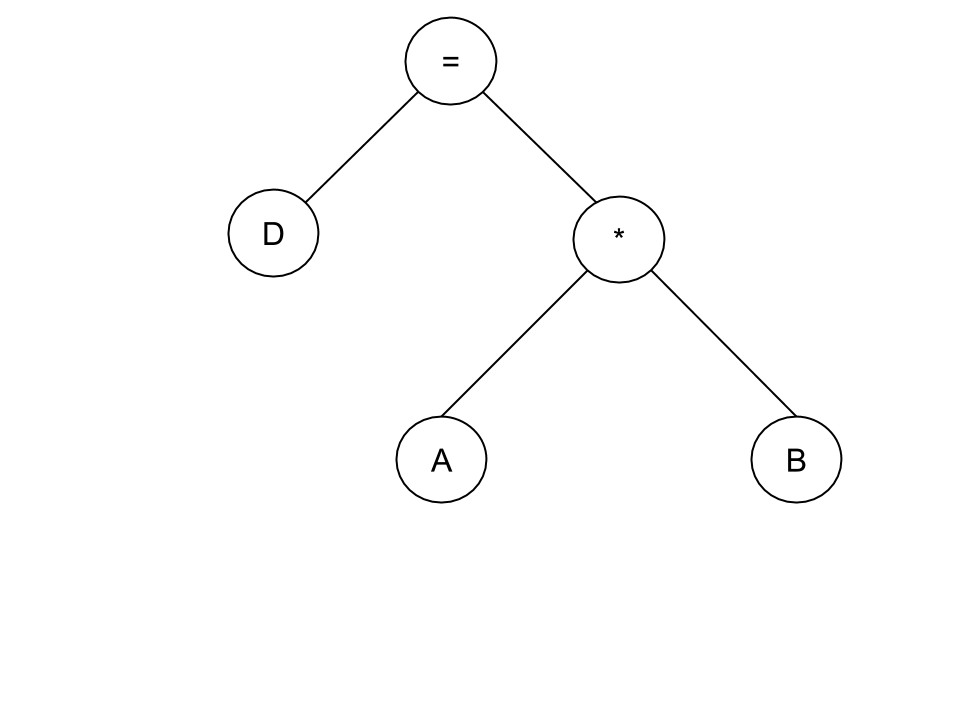
\includegraphics[scale=0.5]{Figures/no_tac.png}
\caption[Statement in \matlab in three address code]{The figure gives an example of an statement in \matlab which is already in three address code and hence is not broken down by Tamer }
\label{Fig:notac}
\end{center}
\end{figure}

In the second case, if the expression is on the LHS, the expression is either a matrix expression or a parameterized expression. In such cases the RHS expression has a temporary variable that is associated with it. The VType for the temporary variable can be generated which will be the VType for the LHS expression. If the expression is on the RHS, the expression itself will have a temporary variable associated with it. \figref{Fig:tac} gives an example of a statement which would be broken down into multiple statements by Tamer. 
\begin{figure}[htbp]
\begin{center}
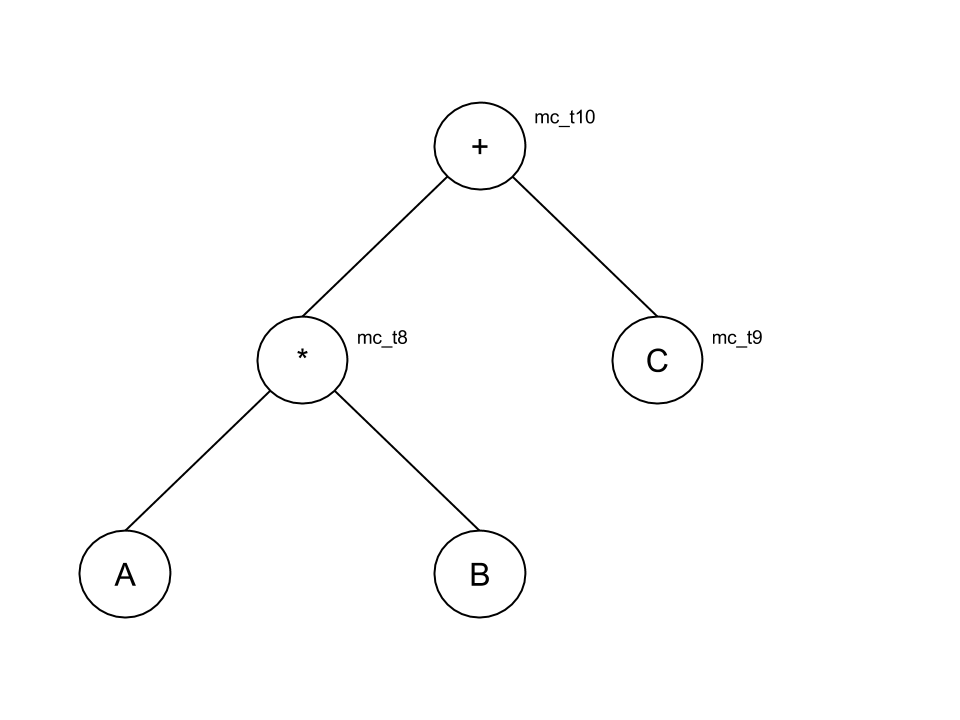
\includegraphics[scale=0.5]{Figures/tac.png}
\caption[Statement in \matlab that is not three address code]{The figure gives an example of an statement in \matlab which is not in three address code and hence is broken down by Tamer using temporaries}
\label{Fig:tac}
\end{center}
\end{figure}
As we can observe each sub-expression has a temporary variable to which it is assigned. The output of the plus expression is assigned to the variable \textsf{mc\_t10} and the output of the multiplication expression is assigned to \textsf{mc\_t8}. The type, shape and whether the expressions are real or complex can be determined by fetching the same information for the temporaries from the analyses. 
\section{Colon Expression transformation}
\label{sec:colonExpr}
The colon expression in \matlab is used in index operations when all the elements of one or more dimensions have to be specified. Listing \ref{lst:colonExprEx} gives an example of an index operation with a colon expression. The second index of the index operation on array A, is a colon expression. The colon expression selects all the column of the array A. For every column index, the element in row 1 is selected. Thus, the index operation will fetch that all values from all the column that are in the first row. Note that we are assuming that the A is a matrix. If the number of dimensions are greater than 2 (greater than the number of indices), the stop value for the colon expression is the product of all the dimension sizes starting from the second dimension. We call this as array dimension flattening. 
\begin{lstlisting}[language=matlab, label={lst:colonExprEx}, caption={An example of the an array index operation with a colon expression as an index. }]
... = A(1,:);
\end{lstlisting}
In this case, if there are 3 dimensions in total, the stop value of the colon expression will be the product of the sizes of the second and the third dimensions. 

There is no equivalent statement in VRIR. In order to generate a range, we need the start and stop values. The start value will always be one. In order to fetch the stop value, we implemented a tranformation which inserts the code to calculate the stop value of the colon expression.This tranformation takes into account that an dimensions will have to be flattened if the the colon expression appears as the last index of of the array index operation. 

We insert a statement before the index operation which stores the size of the dimensions for which the colon expression appears. If the colon expression appears as the last index of the array index operation, we also insert a for loop which takes a product of all the dimension sizes starting from the index position where the colon expression appears to the last dimension of the array. The colon expression is then replaced by range expression with the start value as 1 and the stop value as the calculated size. The range expression can then be compiled to the range described in Subsection \ref{subsec:range}. Table \ref{tab:colonExpr} gives an example of how the McSAF IR is transformed. The first column shows the pretty printed McSAF code before the transformation and the second column shows the pretty printed McSAF after the transformation. The code contains three array index operations, each of which have a colon expression. Since for all three index operations the colon expression appears as the last index, a for loop is also inserted which flattens the array dimensions should the number of dimensions be greater than the number of indices. Moreover, the colon expression is replaced by the range expression with the start value as one and the stop value the one which was calculated.
\begin{table}[htbp]
\centering
\begin{tabular}{|l|l|}
\hline

McSAF (Before transformation) & McSAF (After transformation)\\
\hline
{
\begin{lstlisting}[language=matlab,frame=none, numbers=none]
dr(:) = (R(jj,: ) - R(ii, :));
\end{lstlisting}
}
&
{
\begin{lstlisting}[language=matlab,frame=none, numbers=none]
dim_temp4 = 1;
for dim_temp5 = (1 : ndims(dr));
	dim_temp4 = (dim_temp4 * 
				size(dr, dim_temp5));
end;
dim_temp6 = 1;
for dim_temp7 = (2 : ndims(R));
	dim_temp6 = (dim_temp6 * 
				size(R, dim_temp7));
end;
dim_temp8 = 1;
for dim_temp9 = (2 : ndims(R));
	dim_temp8 = (dim_temp8 * 
				size(R, dim_temp9));
end;
dr((1 : dim_temp4)) = (R(jj, (1 : dim_temp6)) - 
					   R(ii, (1 : dim_temp8)));
\end{lstlisting}

}
 \\
\hline
\end{tabular}
\caption[Example of the colon to range expression transformation]{The table gives an example of the transformation from the colon expression to a range expression. }
\label{tab:colonExpr}
\end{table}
